\documentclass[12pt, twoside]{article}
\usepackage[letterpaper, margin=1in, headsep=0.5in]{geometry}
\usepackage[english]{babel}
\usepackage[utf8]{inputenc}
\usepackage{amsmath}
\usepackage{amsfonts}
\usepackage{amssymb}
\usepackage{tikz}
\usetikzlibrary{quotes, angles}
\usepackage{graphicx}
\usepackage{enumitem}
\usepackage{multicol}
\usepackage{hyperref}

\newif\ifmeta
\metatrue %print standards and topics tags

\title{IB Mathematics}
\author{Chris Huson}
\date{February 2022}

\usepackage{fancyhdr}
\pagestyle{fancy}
\fancyhf{}
\renewcommand{\headrulewidth}{0pt} % disable the underline of the header
\raggedbottom


\fancyhead[LE]{\thepage}
\fancyhead[RO]{\thepage \\ Name: \hspace{4cm} \,\\}
\fancyhead[LO]{BECA / IB Math 5 Exponential functions \\* 16 February 2022}

\begin{document}

\subsubsection*{5.3 Classwork: Exponential function bases}
I can calculate simple interest \hfill CCSS.HSF.IF.C.7

\begin{enumerate}
\item Do Now: Simplify each expression to the base raised to a power.
    \begin{multicols}{2}
    \begin{enumerate}[itemsep=0.5cm]
        \item $5^2 \times 5^4$
        \item $\displaystyle \frac{11^7}{11^5}$
        \item $a^5 \times a^3$
        \item $\displaystyle \left( \frac{x^6}{x^4}\right)^{3}$
    \end{enumerate}
    \end{multicols}

\item A bank account earns interest at an annual interest rate of 3.925\%. The initial deposit is \$175. Which equation models the value of the balance?
\begin{multicols}{2}
    \begin{enumerate}[itemsep=0.5cm]
        \item $FV=175 \cdot 3.925^{t}$
        \item $FV=175 (1+0.03925)^{t}$
        \item $\displaystyle FV=175 \cdot \left( \frac{3.925}{100}\right)^{t}$
        \item $FV=175 \cdot e^{0.03925t}$
    \end{enumerate}
\end{multicols}

\item Carlos puts \$12,500 into an investment account with an annual interest rate of 3.15\% what is the balance after 5 years? \vspace{2cm}

\item The graph shows the exponential function $\displaystyle FV=1,250 \times \left( 1+\frac{4.25}{100} \right)^t$ representing the balance of an investment account earning a fixed rate of interest over $t$ in years.
\begin{multicols}{2}
    \begin{enumerate}[itemsep=1cm]
        \item Write down the initial deposit in the account.
        \item How much will the account hold at the end of ten years, to the nearest \$000?
        \item When will the balance be \$1,600?
    \end{enumerate}
    \begin{center}
    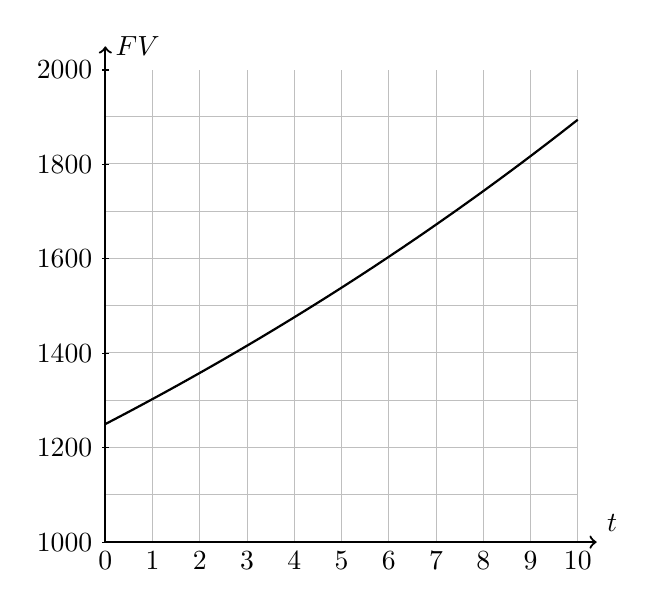
\begin{tikzpicture}[x=1cm, y=0.01cm, scale=0.6]
        \draw [thin, color=lightgray, xstep=1.0cm,ystep=1.0cm] (0,1000) grid (10,2000);
        \draw [thick, ->] (0,1000) -- (+10.4,1000) node [above right]{$t$};
        \draw [thick, ->] (0,1000) -- (0,2050) node [right]{$FV$};        \foreach \x in {0,1,...,10}
            \draw (\x cm,1000) -- (\x cm,1000) node[below] {$\x$};
        \foreach \y in {1000,1200,...,2000}
            \draw[shift={(0,\y)}] (2pt,0pt)--(-2pt,0pt) node[left]{$\y$};

        \draw [thick, smooth,domain=0.:10] plot(\x,{1250*(1.0425^\x)});
    \end{tikzpicture}
    \end{center}
    \end{multicols}

\newpage
\subsubsection*{5.3 Exit Note: Simple interest rates}
\item An asset depreciates at a constant percentage rate, losing $5\%$ of its value each year. The asset's value is modeled by the exponential function $\displaystyle FV=2,000 \times \left( 1-\frac{5}{100} \right)^t$, shown below, where $t$ is the time in years.
\begin{multicols}{2}
    \begin{enumerate}[itemsep=1cm]
        \item Write down the initial value of the asset.
        \item How much will the asset be valued at the end of ten years, to the nearest \$000?
        \item When will the asset have lost one-quarter of its value?
    \end{enumerate}
    \begin{center}
    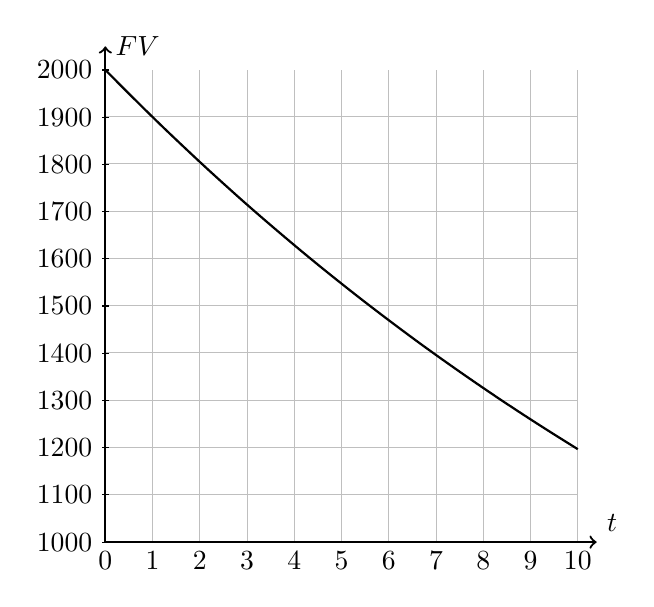
\begin{tikzpicture}[x=1cm, y=0.01cm, scale=0.6]
        \draw [thin, color=lightgray, xstep=1.0cm,ystep=1.0cm] (0,1000) grid (10,2000);
        \draw [thick, ->] (0,1000) -- (+10.4,1000) node [above right]{$t$};
        \draw [thick, ->] (0,1000) -- (0,2050) node [right]{$FV$};        \foreach \x in {0,1,...,10}
            \draw (\x cm,1000)--(\x cm,1000) node[below] {$\x$};
        \foreach \y in {1000,1100,...,2000}
            \draw[shift={(0,\y)}] (2pt,0pt)--(-2pt,0pt) node[left]{$\y$};
        \draw [thick, smooth,domain=0.:10] plot(\x,{2000*(0.95^\x)});
    \end{tikzpicture}
    \end{center}
    \end{multicols}

\item Maria purchases an investment property for \$100,000. Under a special benefit in the tax code, she is allowed to depreciate the asset at $10\%$ annually. 
\begin{enumerate}[itemsep=1cm]
    \item How much can she deduct from her income for tax purposes the first year?
    \item Write an algebraic expression to model the depreciated value of Maria's property.
    \item If she holds it for three years, at what value will it be held on her books?
    \item Make a sketch to represent the graph of the asset's depreciated value over ten years. \vspace{3cm}
    \item She plans to sell the property when it is depreciated to one-half of the purchase value. Find the number of years she expects to hold the property and mark that point on your sketch.
\end{enumerate}
\vspace{2cm}



\end{enumerate}
\end{document}



